\documentclass{article}
\usepackage[UTF8]{ctex}
\usepackage{pythonhighlight}

% Language setting
% Replace `english' with e.g. `spanish' to change the document language
\usepackage[english]{babel}
\usepackage{float}
% Set page size and margins
% Replace `letterpaper' with `a4paper' for UK/EU standard size
\usepackage[letterpaper,top=2cm,bottom=2cm,left=3cm,right=3cm,marginparwidth=1.75cm]{geometry}

% Useful packages
\usepackage{amsmath}
\usepackage{graphicx}
\usepackage[colorlinks=true, allcolors=blue]{hyperref}

\title{进度汇报1}
\author{雷远航}

\begin{document}

\maketitle

\begin{abstract}
第一次进度汇报

\end{abstract}

\section*{一:理论知识学习和一些总结}
目前我主要学习了Computer Vision: Algorithms and Applications书中的第二三章节:Image formation、
Image processing.

在Image formation这一章节中我主要学习了齐次坐标的表示,基于齐次坐标的基本矩阵变换,将这些变换通过opencv
进行了对二维图像的处理,以及关于坐标轴的旋转.同时我也在这一章节中学习了数字摄像机的概念,掌握了一些将三维的图像
投影到二维平面的矩阵变换方法.这一章节包含了很多相关的数学和物理的概念,对这些数理概念也有了一些认识.在练习时我主要
使用了这些方法进行了二维的基本图像变换、以及用数字摄像机投影的原理实现了对空间三角形到二维平面的投影,同时可以绕任意轴进行
旋转.

在Image processing中,我主要学习了各种滤波的方法,图像融合,直方图均衡化,傅立叶变换,和图像金字塔等一些图像处理的方法,并且通过了
opencv对这些处理方法进行了实际的应用.我对这些图像处理的方法的原理有了一定的学习和认识,在excercise中对他们有了一些直观的体会.

由于对opencv的使用一开始还不太熟悉,所以我使用了较为简单的opencv-python进行的处理,本周进行的练习还都比较简单,不过这加深了我对
理论知识的体会,通过简单的python函数接口就可以进行实现.

目前我的学习计划是:2.Image information -> 3.Image processing -> 7.Feature detection and matching -> 8. Image alignment and stitching
-> 11.Structure from motion and SLAM -> 12.Depth estimation -> 13.3D reconstruction 

\section*{二:一些练习}
在这里我只列举了进行的部分练习.

我主要通过了opencv-python,来进行的exercise的实现,主要进行的是对图像的一些处理,目前我进行的练习通过opencv的函数接口实现起来都比较简单,但加深了我对理论
部分知识的学习,并且对这些理论知识有了一些直观的感受.

\subsection*{通过灰度图获取图像边界:}

\begin{figure}[H]
	\centering
	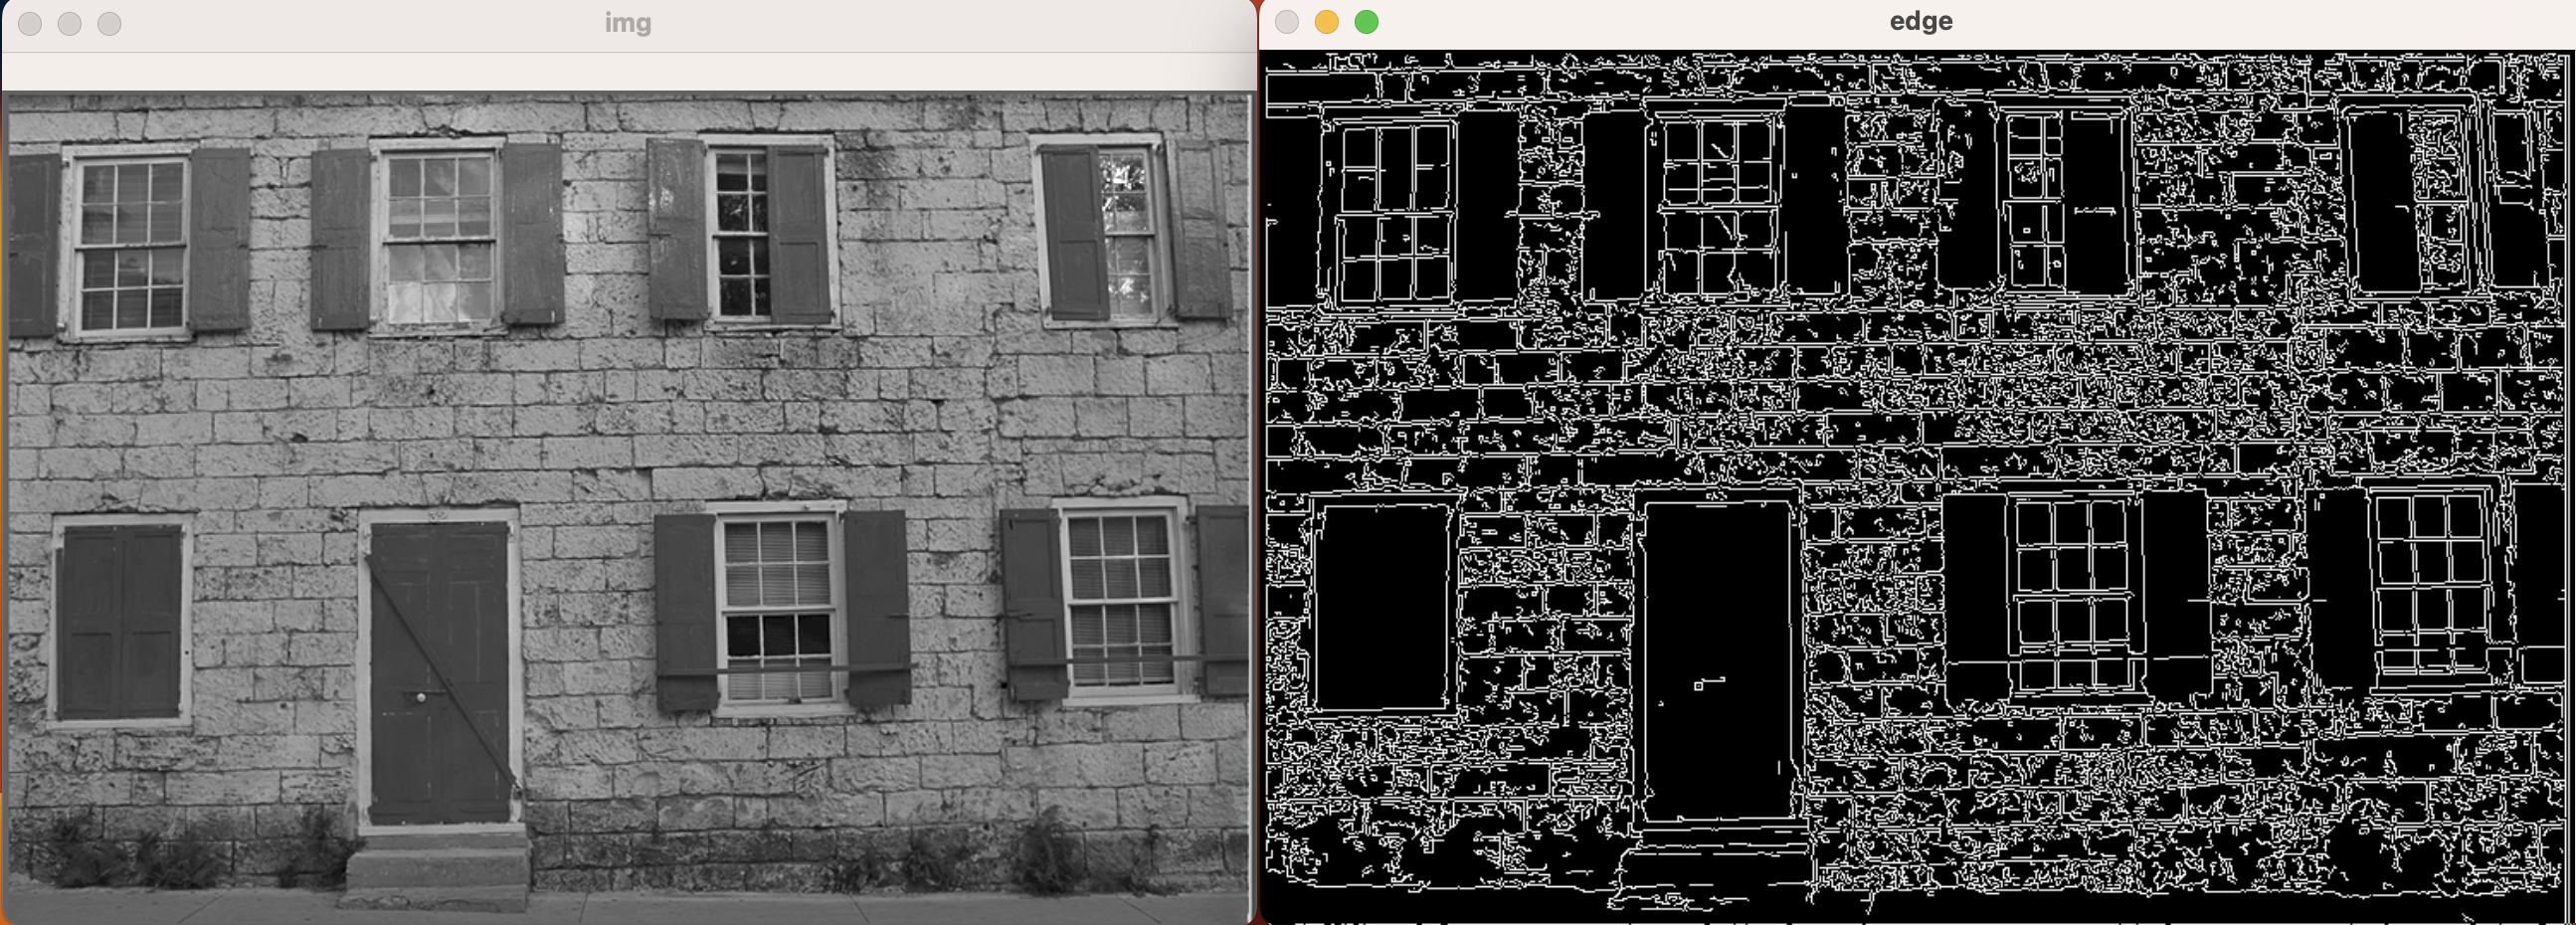
\includegraphics[width=0.7\textwidth]{1.png}
	\caption{\label{pr1}exercise}
	\end{figure}

\subsection*{滤波器应用:}
高通滤波器应用(Laplace,Sobel变换)
\begin{figure}[H]
	\centering
	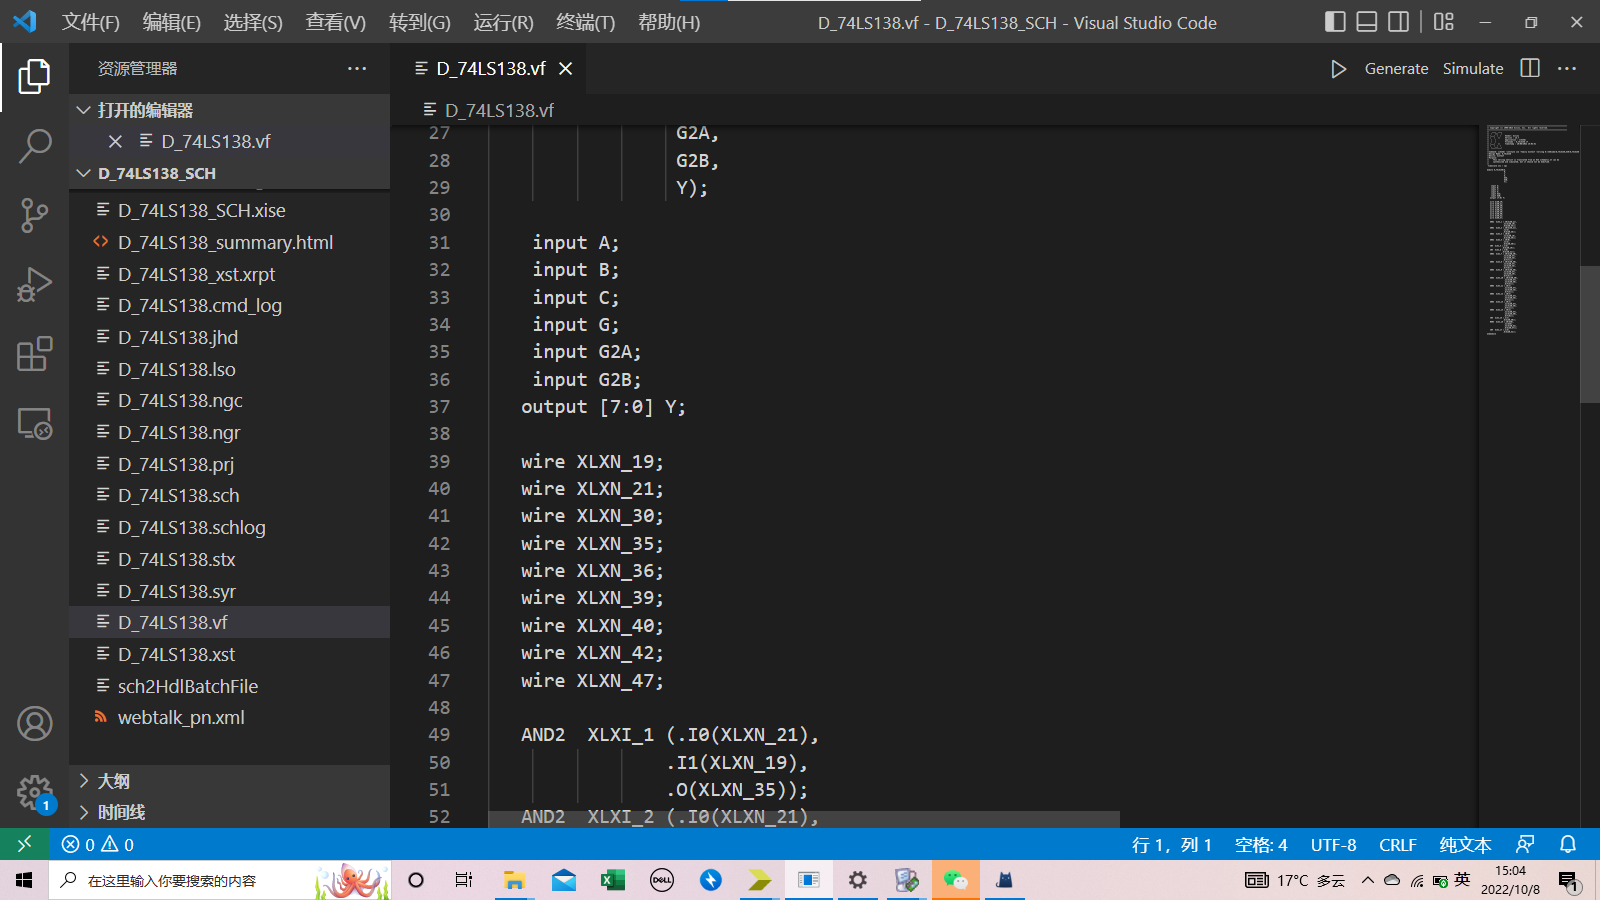
\includegraphics[width=0.7\textwidth]{2.png}
	\caption{\label{pr1}exercise}
	\end{figure}
    
可分离的滤波:
对图像先进行x方向滤波,再进行y方向的滤波与直接一次进行的滤波可以得到相同的结果
\begin{figure}[H]
	\centering
	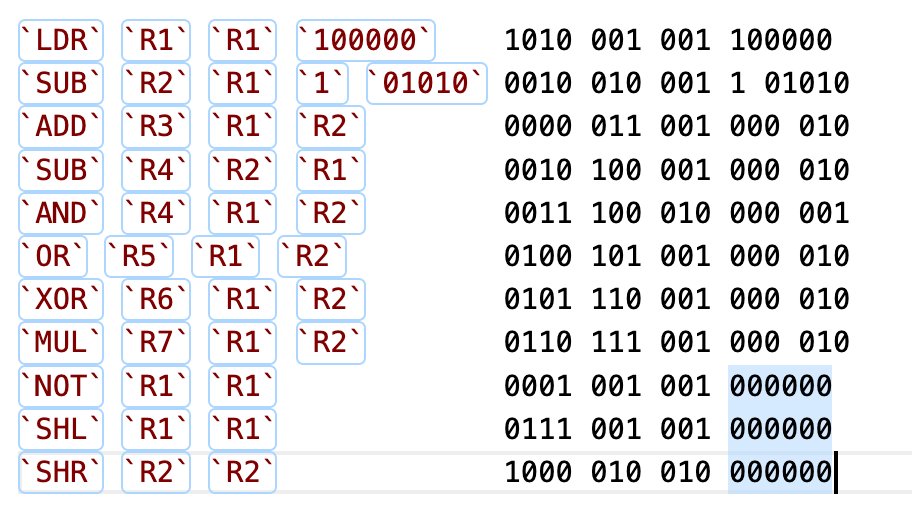
\includegraphics[width=0.7\textwidth]{3.png}
	\caption{\label{pr1}exercise}
	\end{figure}

中位模糊去除椒盐噪声:
\begin{figure}[H]
	\centering
	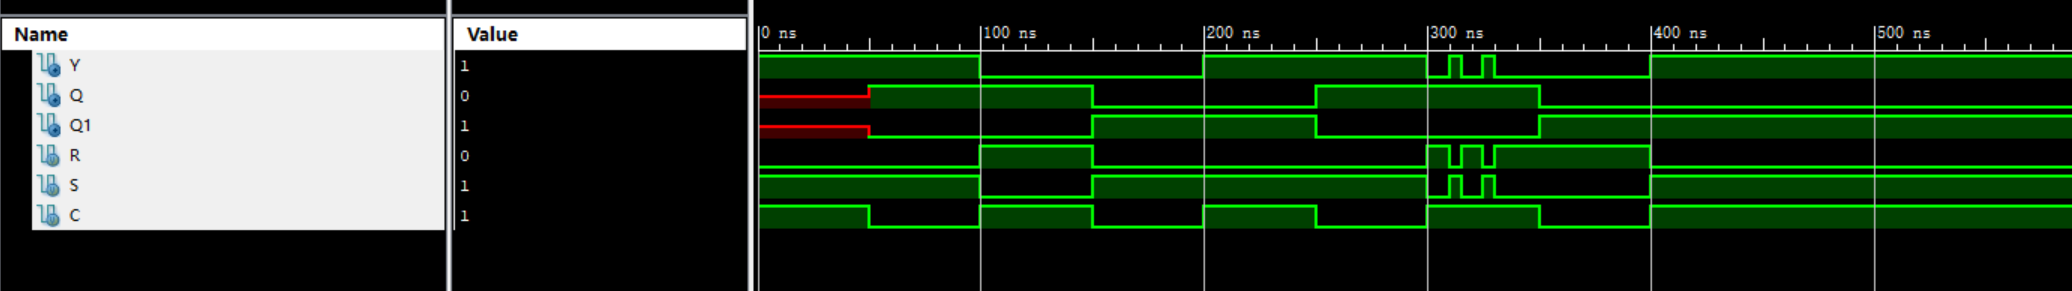
\includegraphics[width=0.7\textwidth]{4.png}
	\caption{\label{pr1}exercise}
	\end{figure}

书中的其他滤波器我也都进行了尝试,在这里不一一列出了.

\subsection*{图像金字塔:}
图像金子塔进行的图像融合:
\begin{figure}[H]
	\centering
	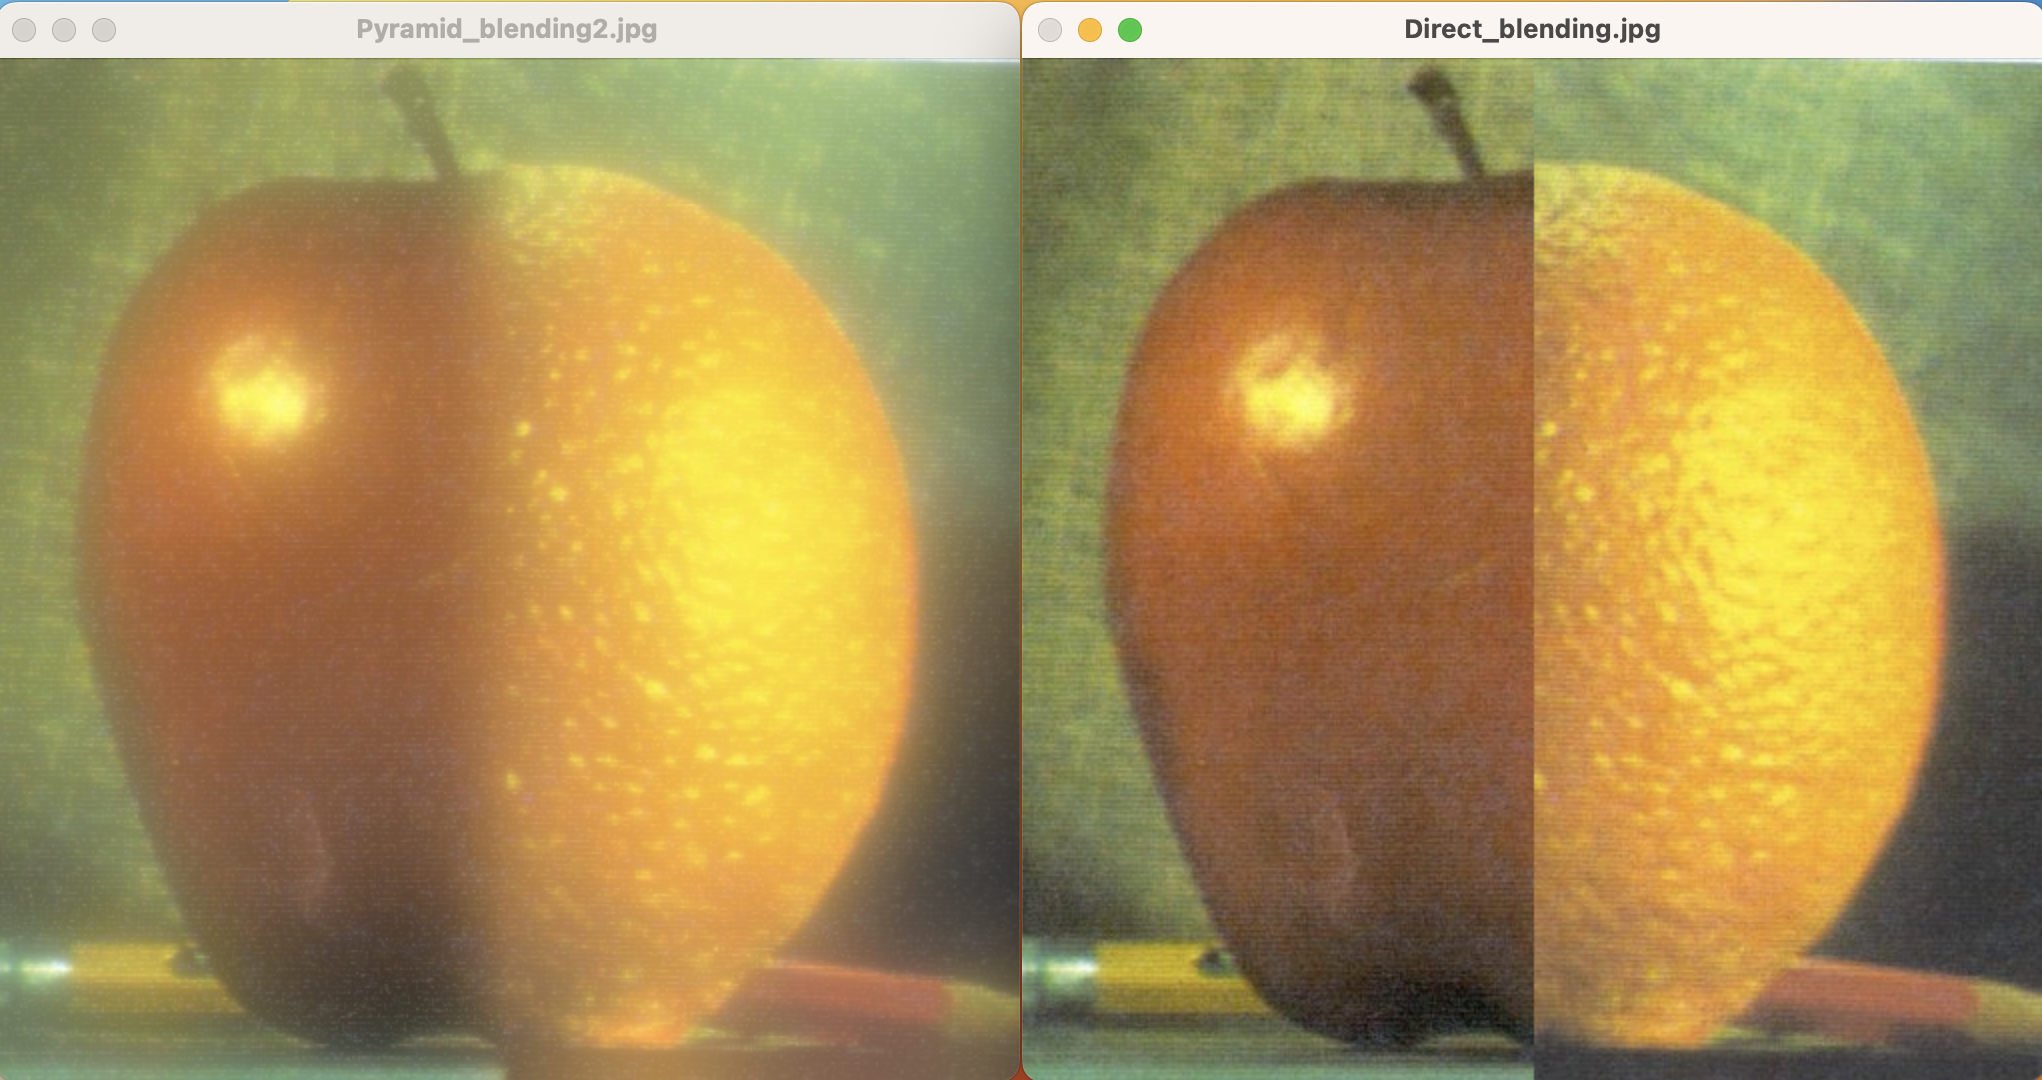
\includegraphics[width=0.7\textwidth]{5.png}
	\caption{\label{pr1}exercise}
	\end{figure}

\subsection*{Fourier变换:}
Fourier变换得到频率图
\begin{figure}[H]
	\centering
	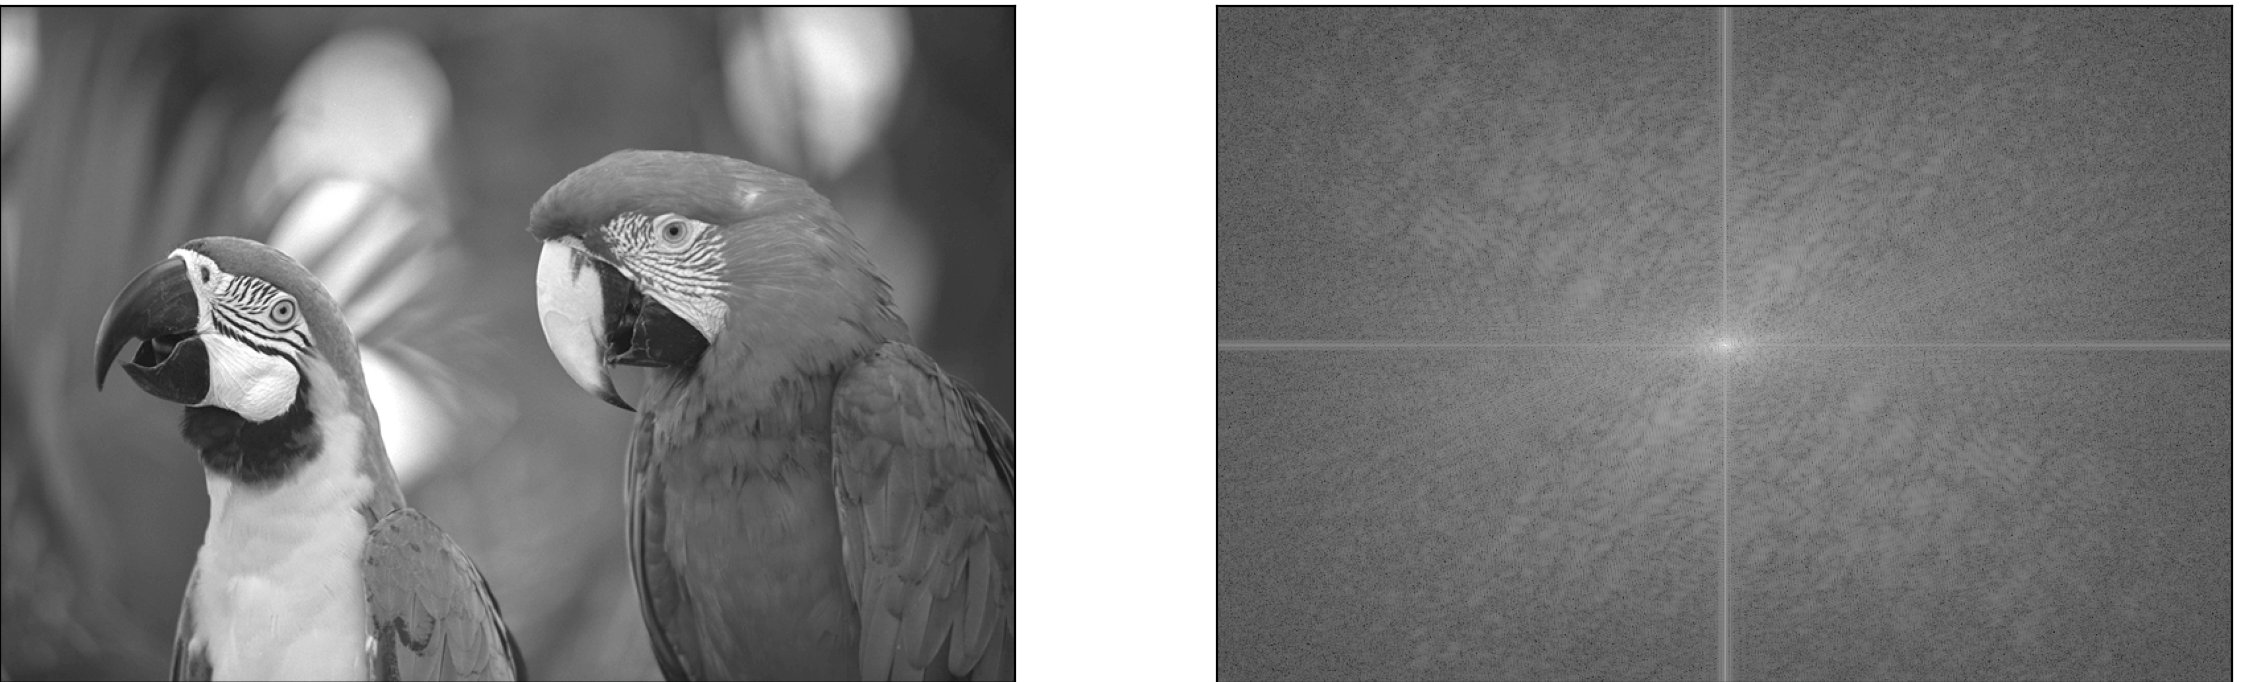
\includegraphics[width=0.7\textwidth]{6.png}
	\caption{\label{pr1}exercise}
	\end{figure}

Fourier变换去除图像低频部分
\begin{figure}[H]
	\centering
	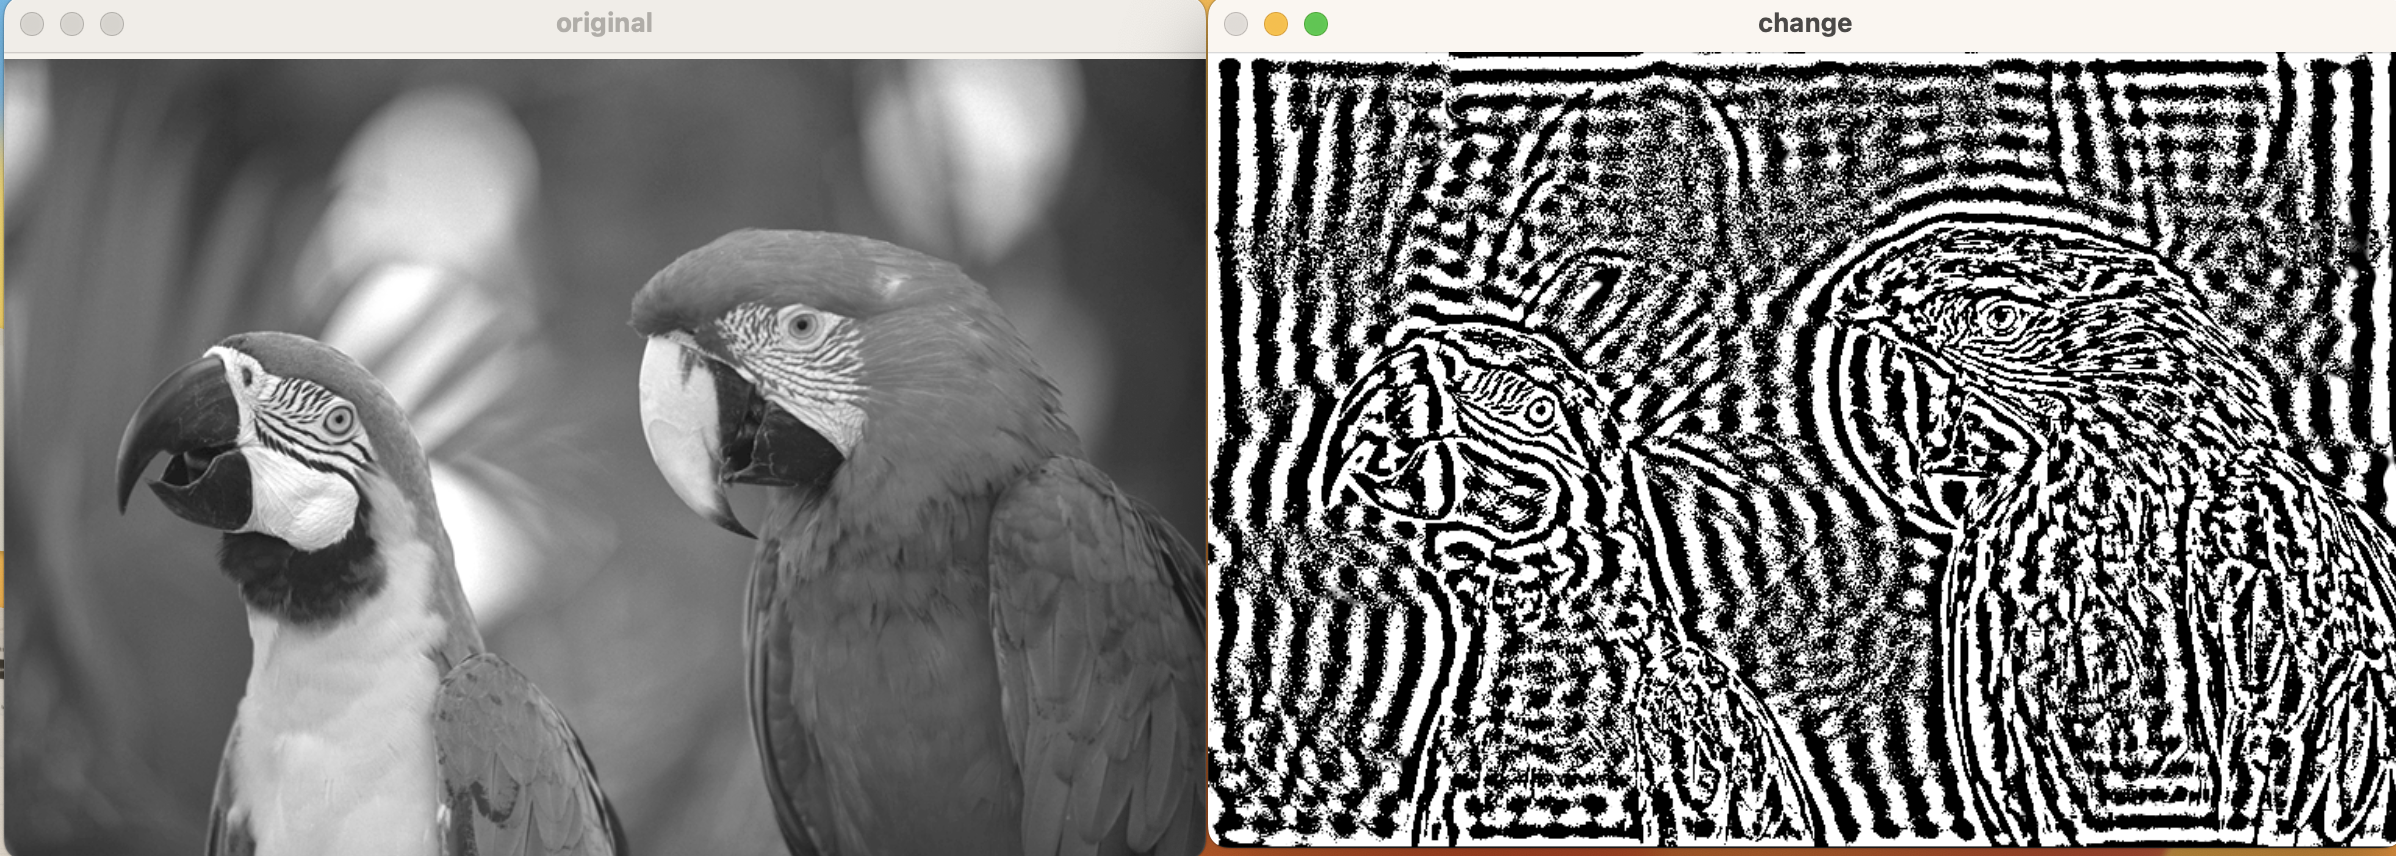
\includegraphics[width=0.7\textwidth]{7.png}
	\caption{\label{pr1}exercise}
	\end{figure}

\subsection*{直方图均衡化:}
通过直方图均衡化增强图像的对比度
\begin{figure}[H]
	\centering
	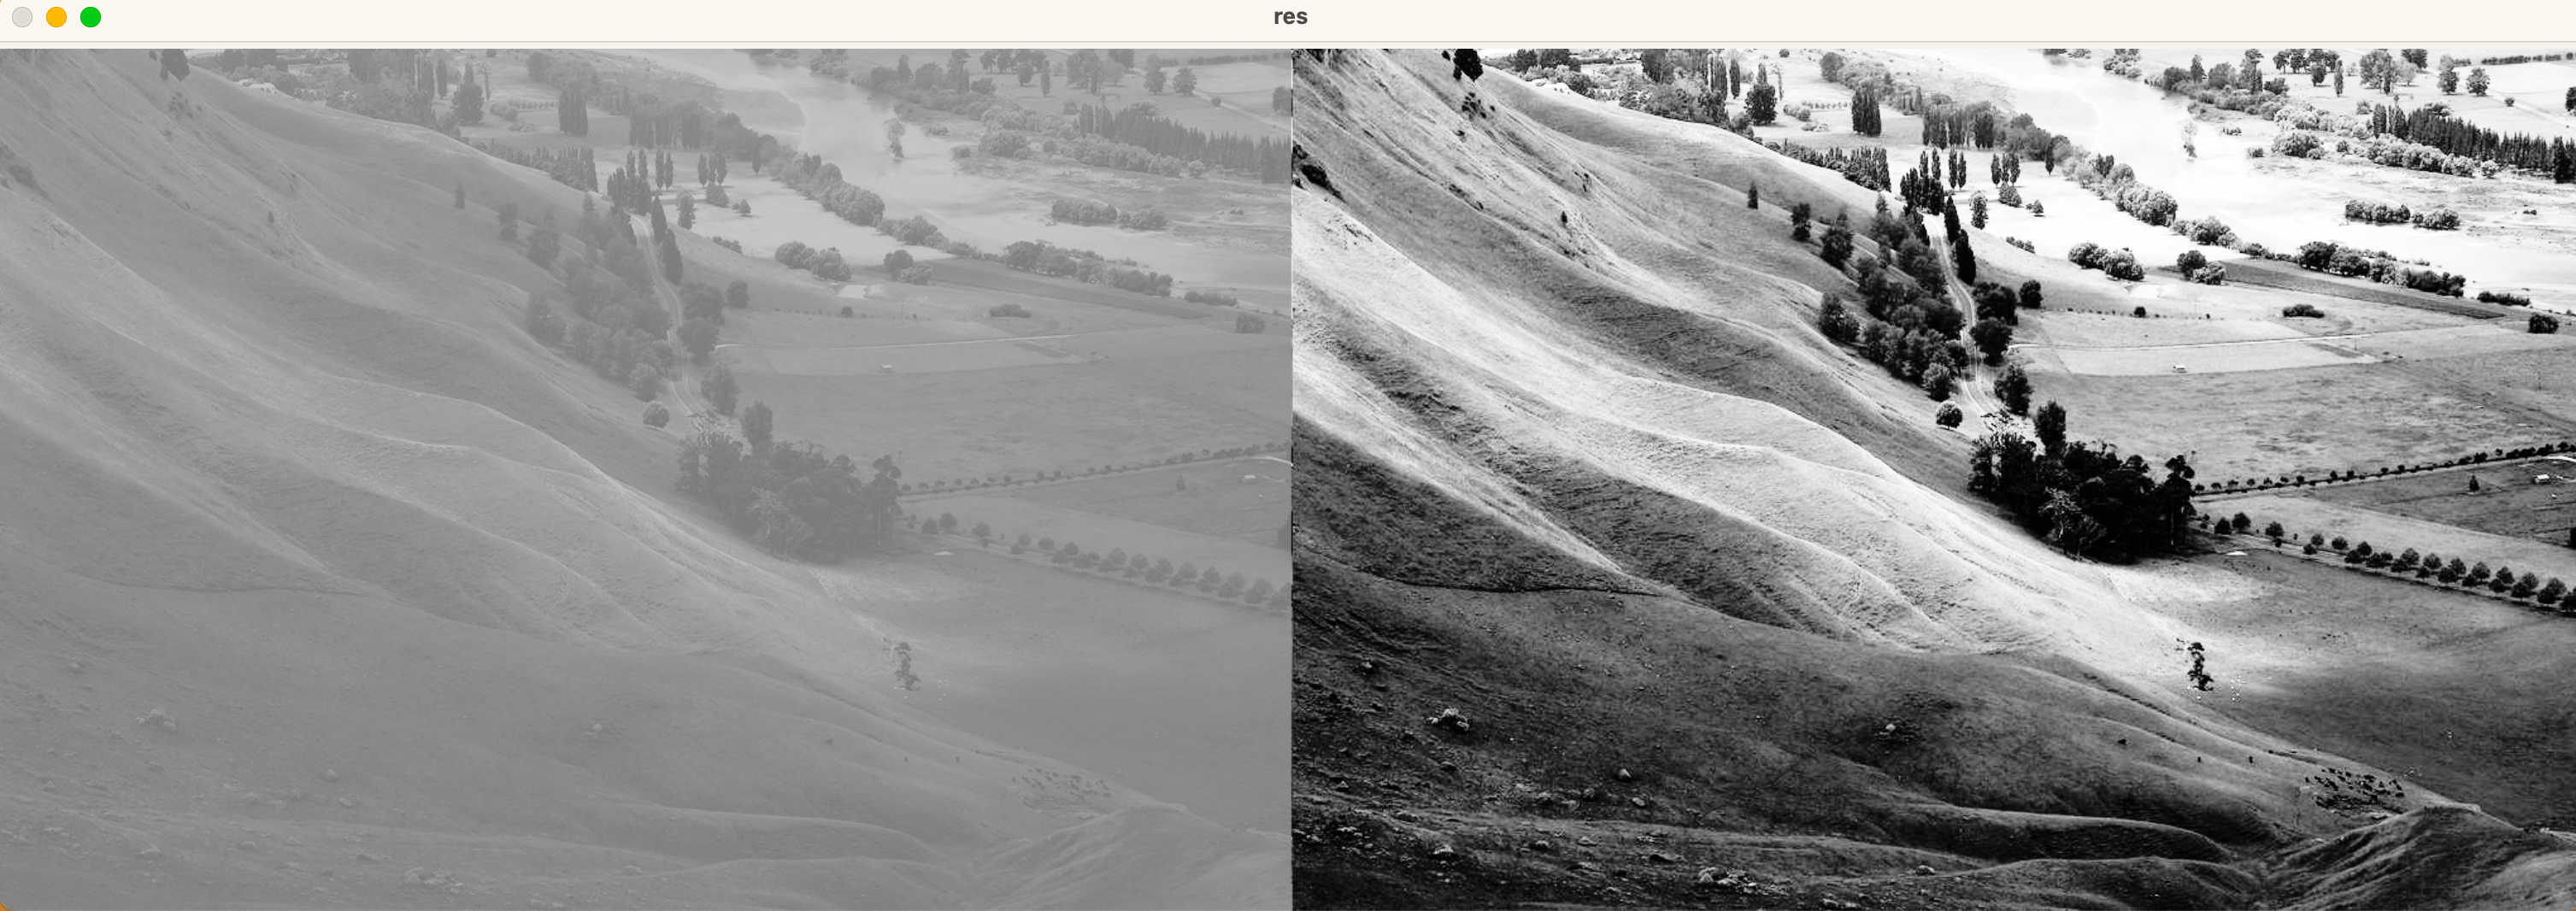
\includegraphics[width=0.7\textwidth]{8.png}
	\caption{\label{pr1}exercise}
	\end{figure}

\subsection*{色彩调整}

通过传入参数对图像的色彩亮度进行变化,通过图像融合的方法可以看到变化的过程

\begin{figure}[H]
	\centering
	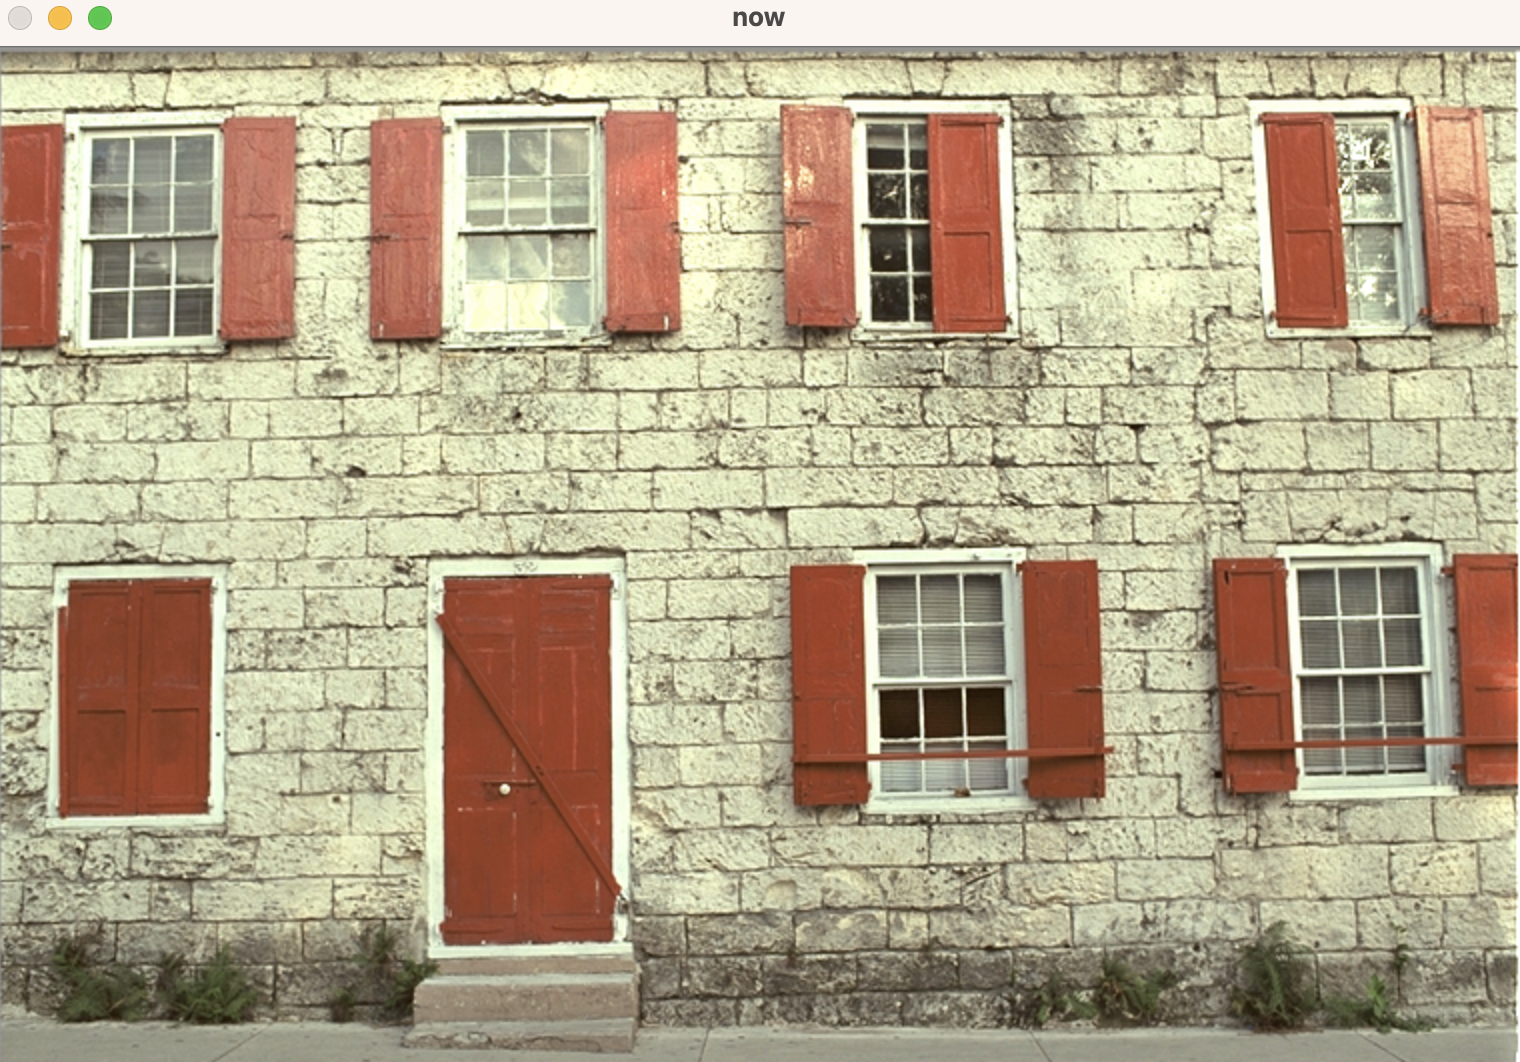
\includegraphics[width=0.7\textwidth]{9.png}
	\caption{\label{pr1}exercise}
	\end{figure}

	\begin{figure}[H]
		\centering
		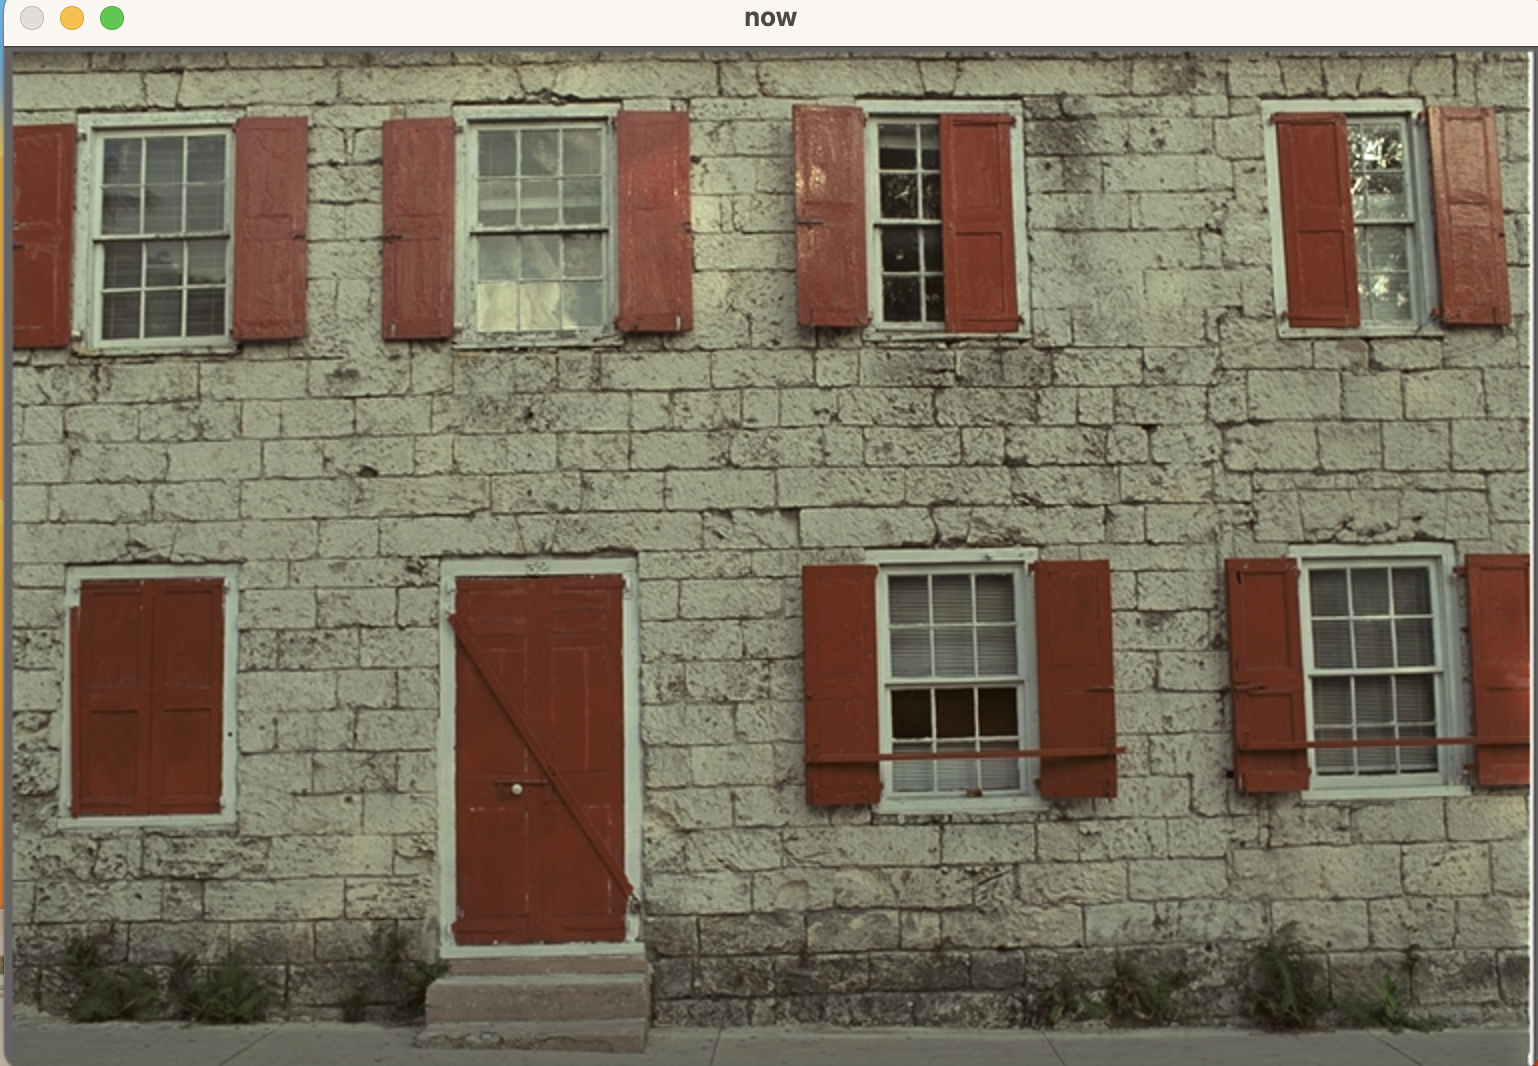
\includegraphics[width=0.7\textwidth]{10.png}
		\caption{\label{pr1}exercise}
		\end{figure}

		\begin{figure}[H]
			\centering
			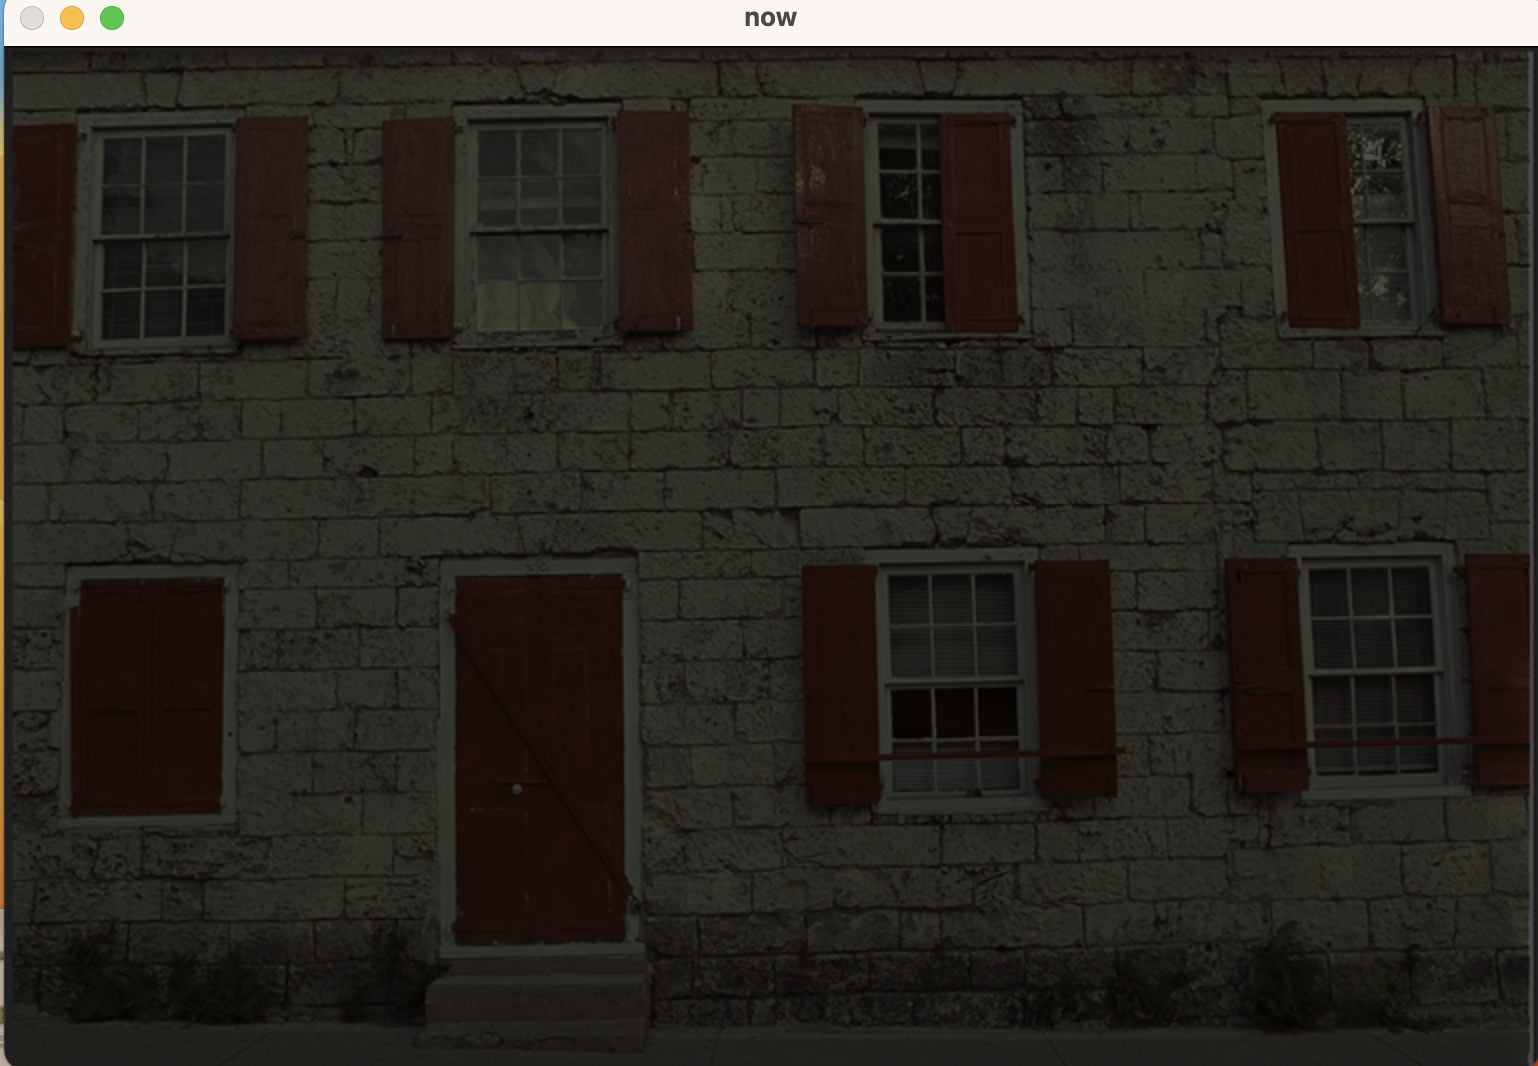
\includegraphics[width=0.7\textwidth]{11.png}
			\caption{\label{pr1}exercise}
			\end{figure}



\end{document}